\subsection{fulibWorkflows Web-Editor Backend}\label{subsec:backend}
Das folgende Kapitel beschäftigt sich mit dem zweiten Bestandteil des Web-Editors, das dazugehörige Backend.
Vom Frontend wird eine YAML-Beschreibung ans Backend geschickt, in diesem wird dies als Eingabe für fulibWorkflows verwendet.
Da fulibWorkflows eine Java-Bibliothek ist, benötigt es ein Backend basierend auf Java.

\subsubsection{Spring Boot}
Mittels \textit{Spring Boot} ist es möglich schnell und ohne zusätzliche Kofniguration eine auf \textit{Spring} basierende Applikation zu erstellen.\cite*{springBoot}
Spring ist ein Framework, welches sich als Ziel gesetzt hat Java Programmierung zu vereinfachen und zu verschnelleren, allerdings keine Einbußen
bei Geschwindikeit, Komplexität und Produktivität zu machen.\cite*{spring}
In diesem Kapitel wird sich mit der Erstellung eines Rest-Services eingegangen.
Ein Rest-Services stellt Endpunkte bereit, welche über REST angesprochen werden können.
Diese eignen sich zur Nutzung als simples Backend.

\begin{figure}[h]
    \centering
    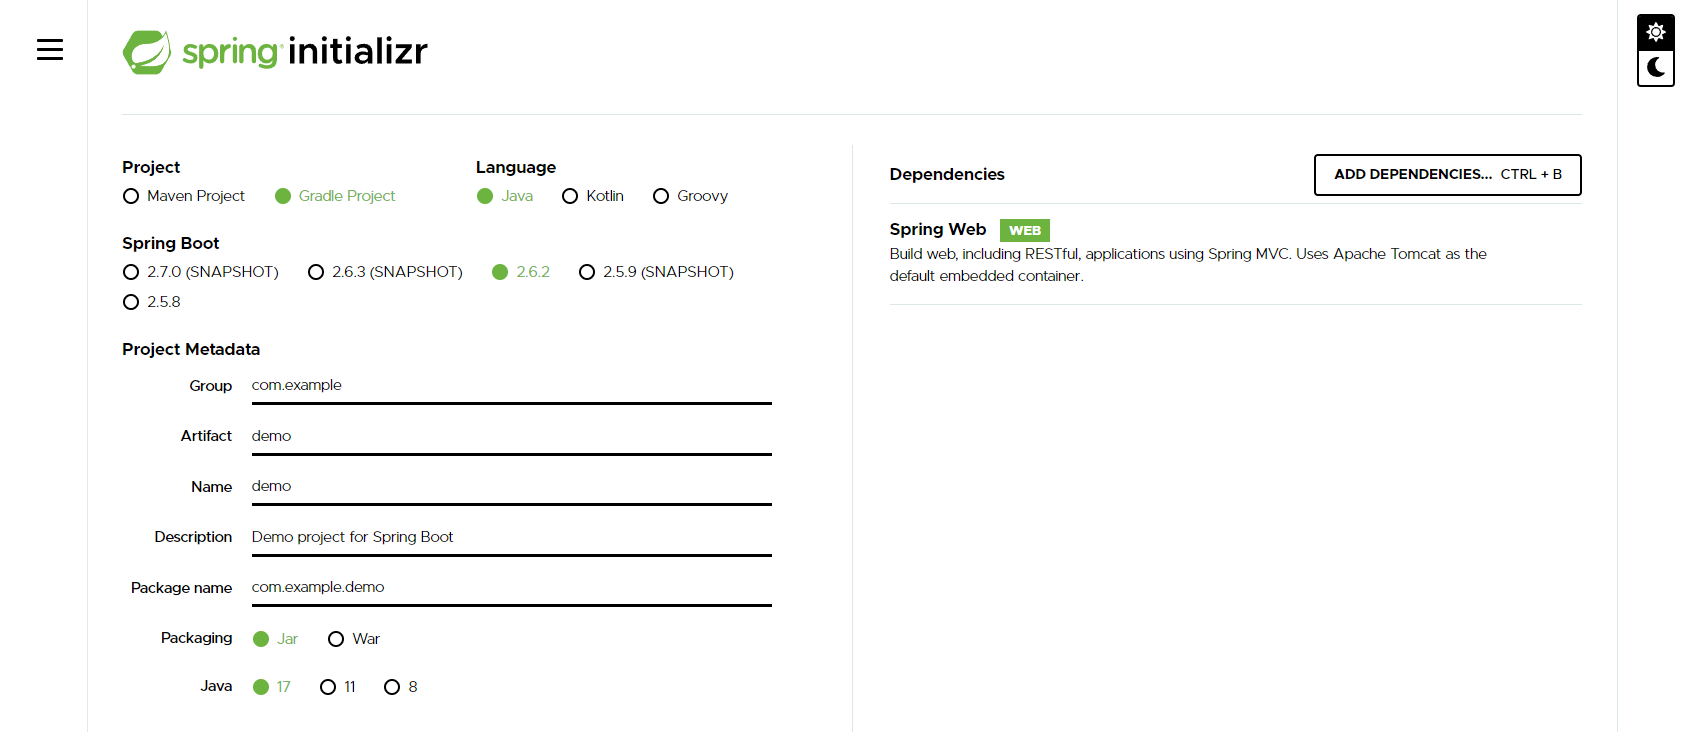
\includegraphics[width=1.0\textwidth]{images/2.2/spring-init}
    \caption{Spring Initalizr für eine Web Anwendung}
    \label{fig:spring-init}
\end{figure}


Das Anlegen eines Spring Boot Projektes kann durch den \textit{Spring Initializr} erledigt werden.\cite*{sbinit}
In Abbildung~\ref{fig:spring-init} ist dieser zu sehen.
Hierbei können diverse Einstellungen getätigt werden, um das zu generierende Projekt an die Anforderungen des Generierenden anzupassen.
Die Abbildung zeigt die getätigten Einstellungen, um ein Gradle Projekt mit Java, Version 17, als Programmiersprache zu generieren.
Ebenfalls kann die Version von Spring Boot eingestellt werden.
Zusätzliche Dependencies können im rechten Bereich des \textit{Spring Initializrs} hinzugefügt werden.
In diesem Fall wurde \textbf{Spring Web} ausgewählt, wodurch die wichtigsten Dependencies für eine REST Applikation bereits enthalten sind.

Das aus den vorherigen Einstellungen beschriebene Projekt ist bereits ein fertiges Backend, welches direkt ausgeführt werden kann.
Durch sogenannte Annotations, welche mit einem @ gekennzeichnet werden, ist es möglich weitere Endpunkte für das Backend zu definieren.
Auf die genaueren Funktionen, welche mittels Annotations implementiert werden können, wird in~\ref{sec:editor-backend} eingegangen, anhand von Beispielen der Implementierung.

